\documentclass{beamer}

\mode<presentation>
{
  \setbeamertemplate{background canvas}[vertical shading][bottom=red!10,top=blue!10]
  \setbeamertemplate{blocks}[rounded][shadow=true]
  \usetheme{Warsaw}
  \setbeamercovered{transparent}
  \usefonttheme[onlysmall]{structurebold}
}


\usepackage[english]{babel}
\usepackage[latin1]{inputenc}
\usepackage{times}
\usepackage[T1]{fontenc}
\usepackage{listings}
\lstloadlanguages{Perl,bash,HTML,XML}
\lstset{language=Perl, numbers=left, numberstyle=\tiny, stepnumber=1, numbersep=5pt,
        frame=lines, captionpos=b, basicstyle=\ttfamily\tiny, breaklines=true}


\title{Introduction to Web Programming with Perl}
\author{Yubao Liu \\ \texttt{yubao.liu@gmail.com}}
\date{2010-11-22}


\hypersetup{pdfpagemode=FullScreen}
\subject{Introduction to Web Programming with Perl}

%\pgfdeclareimage[height=0.5cm]{yahoo-logo}{yahoo-logo.jpg}
%\logo{\pgfuseimage{yahoo-logo}}

\AtBeginSubsection[]
{
  \begin{frame}<beamer>{Outline}
    \tableofcontents[currentsection,currentsubsection]
  \end{frame}
}


\begin{document}

\begin{frame}
  \titlepage
\end{frame}

\begin{frame}{Outline}
  \tableofcontents
  % You might wish to add the option [pausesections]
\end{frame}


\section{Concept}

\subsection{HTTP Protocol}

\begin{frame}{The Data Flow and Format}
  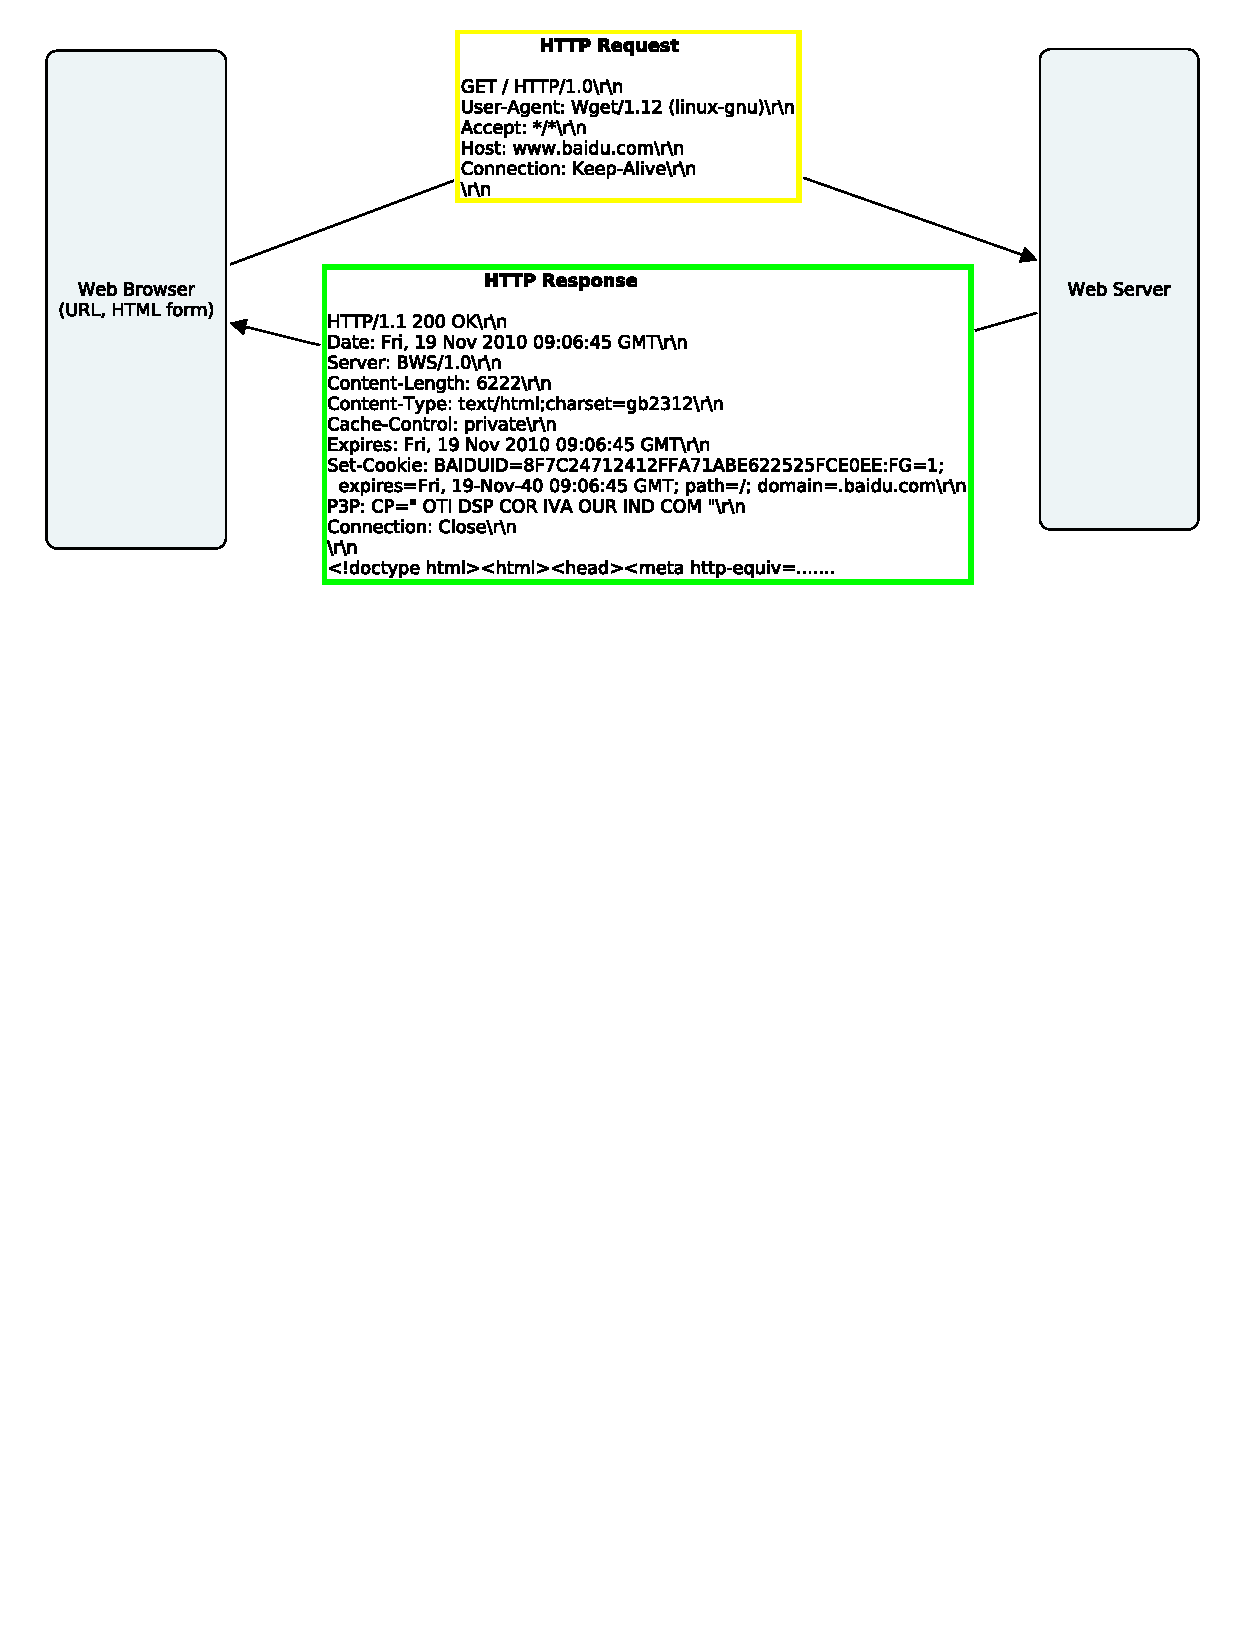
\includegraphics[height=15cm]{data-flow-format}
\end{frame}

\begin{frame}{HTTP Methods}
  \begin{itemize}
    \item GET
    \item POST
    \item PUT
    \item DELETE
    \item HEAD
    \item OPTIONS
    \item CONNECT
    \item TRACE
  \end{itemize}
\end{frame}

\begin{frame}[containsverbatim]{HTTP Method - GET}
  \begin{center}
    \lstinline[language=bash]{wget -d -O - http://www.baidu.com/s?wd=perl+cgi}
  \end{center}
  \begin{lstlisting}[language=, caption=HTTP request using GET method]
GET /s?wd=perl+cgi HTTP/1.0\r\n
User-Agent: Wget/1.12 (linux-gnu)\r\n
Accept: */*\r\n
Host: www.baidu.com\r\n
Connection: Keep-Alive\r\n
\r\n
  \end{lstlisting}
\end{frame}

\begin{frame}[containsverbatim]{HTTP Method - POST}
 \lstinputlisting[language=HTML, caption=HTML form with POST method]{hello.html}
\end{frame}

\begin{frame}[containsverbatim]{HTTP Method - POST (cont.)}
  \begin{lstlisting}[language=, caption=HTTP request using POST method]
POST /~liuyb/cgi-bin/hello.cgi HTTP/1.1\r\n
Host: localhost\r\n
User-Agent: Mozilla/5.0 (X11; U; Linux i686; en-US; rv:1.9.1.13) Gecko/20100916 Iceweasel/3.5.13 (like Firefox/3.5.13)\r\n
Accept: text/html,application/xhtml+xml,application/xml;q=0.9,*/*;q=0.8\r\n
Accept-Language: en-us,en;q=0.5\r\n
Accept-Encoding: gzip,deflate\r\n
Accept-Charset: ISO-8859-1,utf-8;q=0.7,*;q=0.7\r\n
Keep-Alive: 300\r\n
Connection: keep-alive\r\n
Referer: http://localhost/~liuyb/hello.html\r\n
Content-Type: application/x-www-form-urlencoded\r\n
Content-Length: 36\r\n
\r\n
name=Anonymous&comment=Your+comment.
  \end{lstlisting}
\end{frame}

\subsection{The Perl Way}

\begin{frame}{The Paradigms}
  \begin{itemize}
    \item Customzied web server
    \item Common web server + external programs
        \begin{itemize}
            \item One shot: CGI
            \item Daemon: FastCGI, SpeedyCGI, SCGI
        \end{itemize}
    \item Common web server + web server plugins
  \end{itemize}
\end{frame}

\begin{frame}{The Perl Web Stack}
  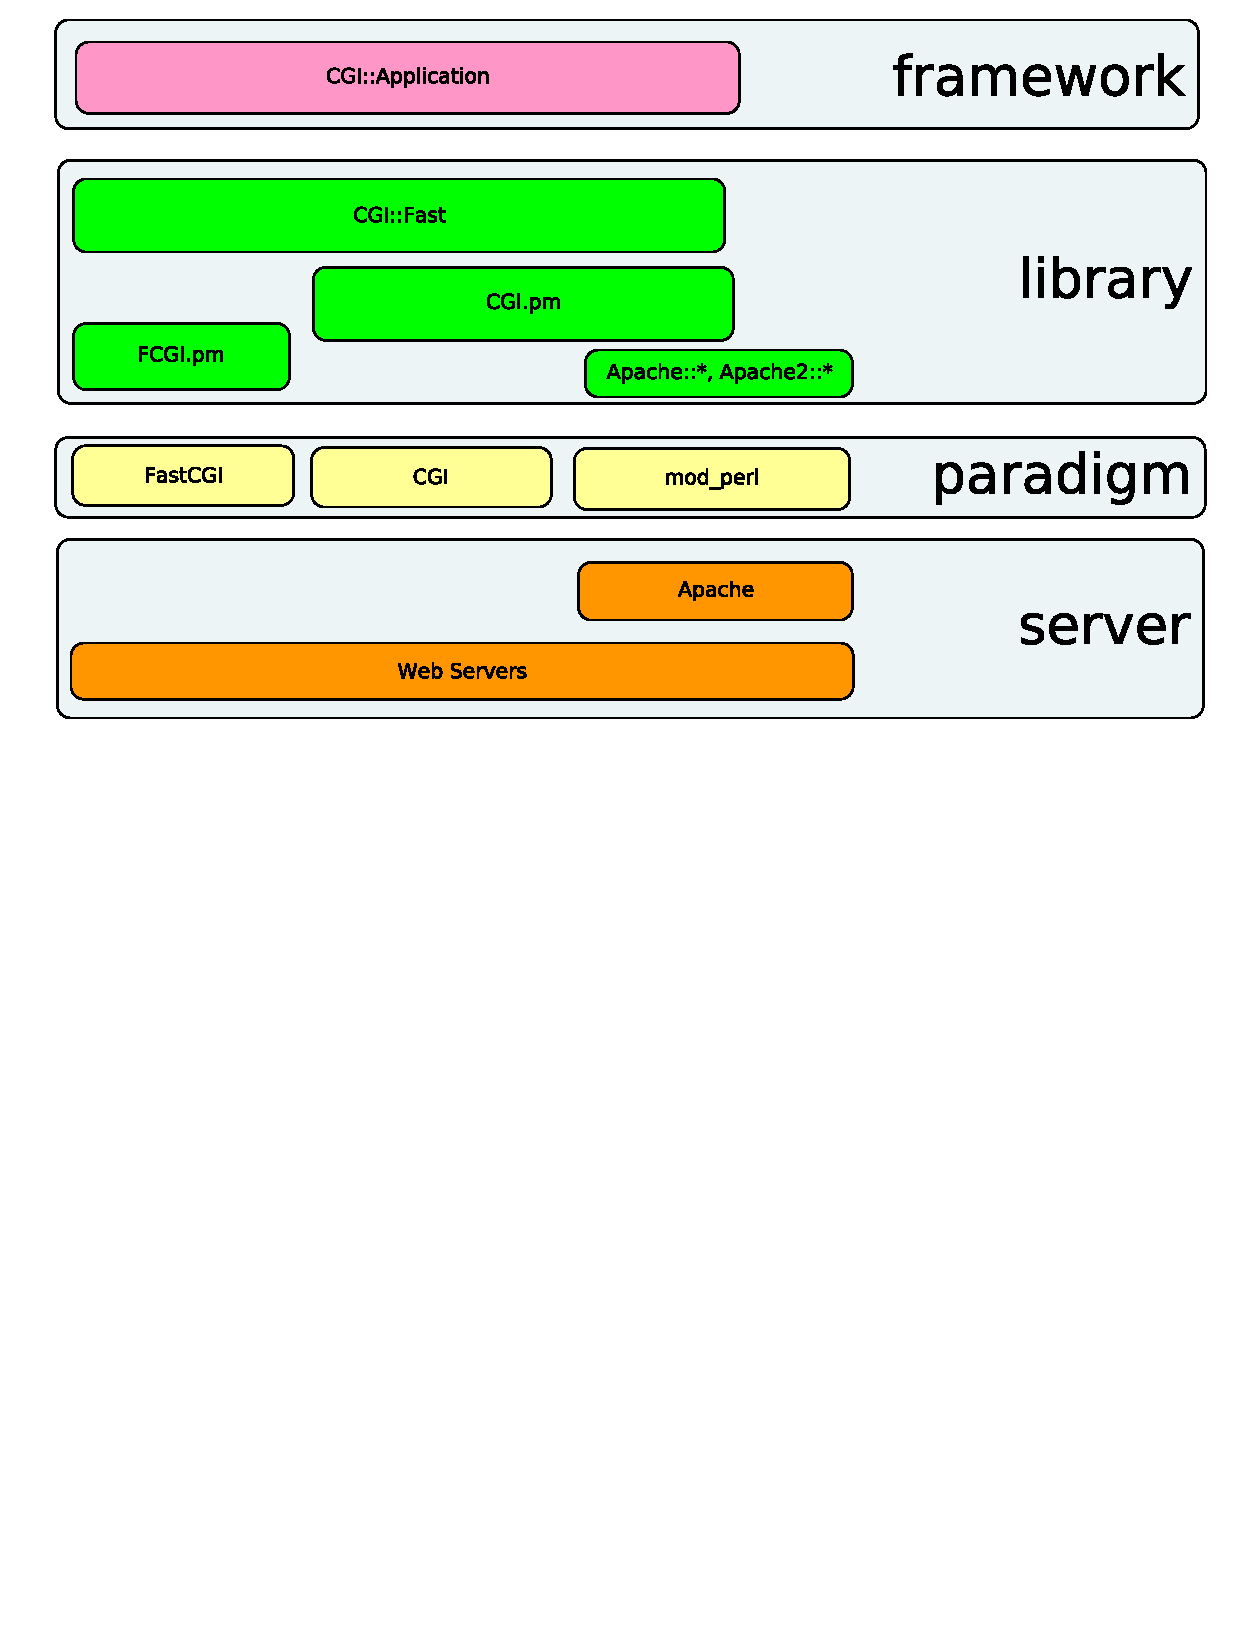
\includegraphics[height=14cm]{perl-web-stack}
\end{frame}

\begin{frame}{The Perl Web Stack (cont.)}
  \begin{itemize}
    \item New foundation: PSGI, Plack
    \item Frameworks: Catalyst, Dance, Mojolicious
    \item Fancy stuffs: Starman, Perlbal, Gearman, HTTP::Server::Simple,
          HTTP::Daemon, Net::Server, POE::Component::Server::HTTP,
          POE::Component::Server::SimpleHTTP, Template::Toolkit, DBI,
          Class::DBI, DBIx::Class, DBIx::Simple, Rose::DB::Object
  \end{itemize}
\end{frame}


\section{Practice}

\begin{frame}
  \begin{center}
    {\Large\emph{Here are fundamental things, \\
            you'd better use high level frameworks!}}
  \end{center}
\end{frame}

\begin{frame}[containsverbatim]{Setup on Debian Squeeze}
  \lstinputlisting[language=bash, caption=Installation]{install.sh}
  \lstinputlisting[language=XML, caption=Configuration]{my-cgi.conf}
\end{frame}

\subsection{CGI}

\begin{frame}[containsverbatim]{CGI Modules}
  \begin{center}
Poor performance.
  \end{center}
  \begin{itemize}
    \item mod\_cgi   (preferred for prefork MPM)
    \item mod\_cgid  (preferred for worker MPM)
  \end{itemize}
\end{frame}

\begin{frame}[containsverbatim]{Example CGI Script}
\lstinputlisting[language=Perl, caption=CGI example]{hello.cgi}
\end{frame}

\begin{frame}[containsverbatim]{HTML Template}
\lstinputlisting[language=HTML, caption=HTML template example]{hello.tmpl}
\end{frame}

\subsection{FastCGI}

\begin{frame}{FastCGI Modules}
  \begin{center}
100x faster than CGI, high performance, stable, portable
  \end{center}
  \begin{itemize}
    \item mod\_fastcgi (faster, old, non-free)
    \item mod\_fcgid   (more stable, actively maintained)
  \end{itemize}
\end{frame}

\begin{frame}[containsverbatim]{Example FastCGI Script}
\lstinputlisting[language=Perl, caption=FastCGI example]{hello.fcgi}
\end{frame}

\subsection{mod\_perl}

\begin{frame}{mod\_perl Modules}
  \begin{center}
100x faster than CGI, high performance, powerful, non-portable
  \end{center}
  \begin{itemize}
    \item mod\_perl 1.x (for Apache 1.x)
    \item mod\_perl 2.x (less features, for Apache 2.x)
  \end{itemize}
\end{frame}

\begin{frame}[containsverbatim]{Example mod\_perl Script}
\lstinputlisting[language=Perl, caption=mod\_perl example]{hello.pl}
\end{frame}

\begin{frame}{More About mod\_perl}
  \begin{itemize}
    \item ModPerl::Registry, ModPerl::PerlRun
    \item PerlPassEnv, PerlSetEnv, PerlModule, PerlRequire, Perl*Handler
          \footnote{\tiny
                \href{http://perl.apache.org/docs/1.0/guide/config.html\#Perl\_Handlers}{mod\_perl 1.x Perl*Handler},
                \href{http://perl.apache.org/docs/2.0/user/config/config.html\#HTTP\_Protocol\_Handlers\_Directives}{mod\_perl 2.x Perl*Handler}}
    \item Apache::*, Apache2::*, ModPerl::*
  \end{itemize}
\end{frame}

\begin{frame}{Traps}
  \begin{itemize}
    \item Relative path
    \item User and group of Apache processes
    \item Executable permission on CGI and FastCGI scripts
    \item Reload Perl modules and scripts after modification
    \item Cache-Control and Expires headers
  \end{itemize}
\end{frame}

\begin{frame}{Traps (cont.)}
  \begin{itemize}
    \item Take care global states, don't presume server processing model
    \item Different parameter acquiring in GET and POST requests
    \item Proper Content-Type and Content-Length headers
    \item Use CGI.pm or other high level modules, don't presume paradigm
  \end{itemize}
\end{frame}

\begin{frame}{Debugging}
  \begin{itemize}
    \item Running on command line, CGI.pm, Apache
    \item CGI::Carp
    \item Apache::Reload, Apache2::Reload, Apache::FakeRequest, Apache::DB
    \item FireBug, Wireshark
  \end{itemize}
\end{frame}

\section{Reference}

\begin{frame}{Useful Materials}
  \begin{itemize}
    \item \href{http://httpd.apache.org/docs/}{http://httpd.apache.org/docs/}
    \item \href{http://perl.apache.org/docs/index.html}{http://perl.apache.org/docs/index.html}
    \item \emph{CGI Programming with Perl}, O'Reilly
    \item \emph{Writing CGI Applications With Perl}, Addison-Wesley Professional
    \item \emph{Practical mod\_perl}, O'Reilly, \href{http://modperlbook.org/}{http://modperlbook.org/}
    \item \emph{mod\_perl2 User's Guide}, OnyxNeon
  \end{itemize}
\end{frame}

\begin{frame}
  \begin{center}
    {\sl \_\_END\_\_}
  \end{center}
\end{frame}

\end{document}

